\section{Objective}
The objective of this project is to build a dynamic robot in order to experiment with reinforcement learning algorithms with real data. We wish to make this experiments easy and cheap to reproduce so we will try minimize its components and fabrication cost. 

The chosen robot is inspired in a \textit{segway hover-board}, similar to the one in Figure \ref{fig:Picture of a commercial segway hover-board}. The two wheels are controlled with classic control algorithms and the inclination of the central body is controlled with a reinforcement learning algorithm.

\begin{figure}
	\centering
	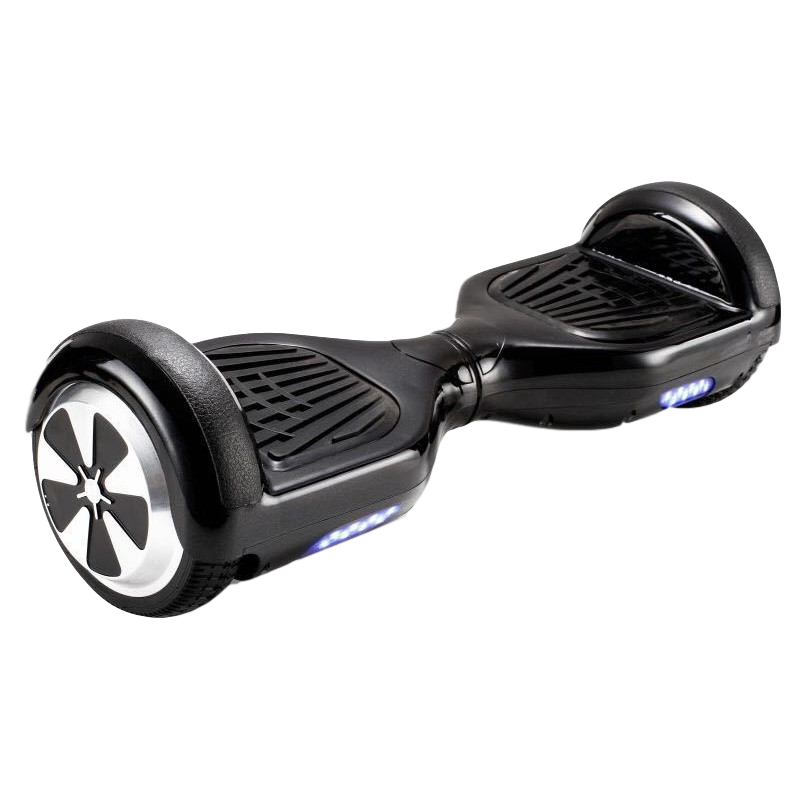
\includegraphics[width=8cm]{img/segway_hoverboard_picture.png}
	\caption{Picture of a commercial \textit{segway hover-board} }
	\label{fig:Picture of a commercial segway hover-board}
\end{figure}